\documentclass[portrait,paperwidth=24in,paperheight=36in,fontscale=0.5]{baposter}

\usepackage{calc}
\usepackage{graphicx}
\usepackage{amsmath}
\usepackage{amssymb}
\usepackage{braket}
\usepackage{relsize}
\usepackage{multirow}
\usepackage{rotating}
\usepackage{bm}
\usepackage{url}
\usepackage{graphicx}
\usepackage{multicol}
\usepackage{algorithm2e}
\usepackage{fancybox}
\usepackage{tikz}

%\usepackage{times}
%\usepackage{helvet}
%\usepackage{bookman}
\usepackage{palatino}

\newcommand{\captionfont}{\footnotesize}

\graphicspath{{Images/}{../}}
\usetikzlibrary{calc}

\newcommand{\ph}{\ensuremath{\varphi}}
\newcommand{\ii}{\ensuremath{\mathrm{i}}}
\newcommand{\lt}{\ensuremath{\widetilde{l}}}
\newcommand{\pt}{\ensuremath{\widetilde{p}}}
%%%%%%%%%%%%%%%%%%%%%%%%%%%%%%%%%%%%%%%%%%%%%%%%%%%%%%%%%%%%%%%%%%%%%%%%%%%%%%%%
%%%% Some math symbols used in the text
%%%%%%%%%%%%%%%%%%%%%%%%%%%%%%%%%%%%%%%%%%%%%%%%%%%%%%%%%%%%%%%%%%%%%%%%%%%%%%%%

%%%%%%%%%%%%%%%%%%%%%%%%%%%%%%%%%%%%%%%%%%%%%%%%%%%%%%%%%%%%%%%%%%%%%%%%%%%%%%%%
% Multicol Settings
%%%%%%%%%%%%%%%%%%%%%%%%%%%%%%%%%%%%%%%%%%%%%%%%%%%%%%%%%%%%%%%%%%%%%%%%%%%%%%%%
\setlength{\columnsep}{1.5em}
\setlength{\columnseprule}{0mm}

%%%%%%%%%%%%%%%%%%%%%%%%%%%%%%%%%%%%%%%%%%%%%%%%%%%%%%%%%%%%%%%%%%%%%%%%%%%%%%%%
% Save space in lists. Use this after the opening of the list
%%%%%%%%%%%%%%%%%%%%%%%%%%%%%%%%%%%%%%%%%%%%%%%%%%%%%%%%%%%%%%%%%%%%%%%%%%%%%%%%
\newcommand{\compresslist}{%
\setlength{\itemsep}{1pt}%
\setlength{\parskip}{0pt}%
\setlength{\parsep}{0pt}%
}

%%%%%%%%%%%%%%%%%%%%%%%%%%%%%%%%%%%%%%%%%%%%%%%%%%%%%%%%%%%%%%%%%%%%%%%%%%%%%%
%%% Begin of Document
%%%%%%%%%%%%%%%%%%%%%%%%%%%%%%%%%%%%%%%%%%%%%%%%%%%%%%%%%%%%%%%%%%%%%%%%%%%%%%

\begin{document}

%%%%%%%%%%%%%%%%%%%%%%%%%%%%%%%%%%%%%%%%%%%%%%%%%%%%%%%%%%%%%%%%%%%%%%%%%%%%%%
%%% Here starts the poster
%%%---------------------------------------------------------------------------
%%% Format it to your taste with the options
%%%%%%%%%%%%%%%%%%%%%%%%%%%%%%%%%%%%%%%%%%%%%%%%%%%%%%%%%%%%%%%%%%%%%%%%%%%%%%
% Define some colors

\definecolor{uscgold}{RGB}{255,204,0}
\definecolor{uscred}{RGB}{153,27,30}
\begin{poster}%
  % Poster Options
  {
  % Show grid to help with alignment
  grid=false,
  columns=2,
  % Column spacing
  colspacing=1em,
  % Color style
  bgColorOne=white,
  bgColorTwo=white,
  borderColor=black,
  headerColorOne=uscred,
  headerColorTwo=uscgold,
  headerFontColor=white,
  boxColorOne=white,
  boxColorTwo=white,
  % Format of textbox
  textborder=roundedleft,
  % Format of text header
  eyecatcher=false,
  headerborder=closed,
  headerheight=0.1\textheight,
%  textfont=\sc, An example of changing the text font
  headershape=roundedright,
  headershade=shadelr,
  headerfont=\Large\bf\textsc, %Sans Serif
  textfont={\setlength{\parindent}{1.5em}},
  boxshade=plain,
%  background=shade-tb,
  background=plain,
  linewidth=2pt
  }% Eye Catcher
  {}
  % Title
  {\bf\textsc{MPI, CUDA, and Quantum Evolution}\vspace{0.5em}}
  % Authors
  {\textsc{Christopher Cantwell \hspace{14.0em} Jose Raul Gonzalez Alonso}\\ \smaller{\texttt{ccantwel@usc.edu\hspace{25.25em jrgonzal@usc.edu}}}}
  % University logo
  {% The makebox allows the title to flow into the logo, this is a hack because of the L shaped logo.
    
\includegraphics[scale=0.2]{Images/USC.pdf}
  }
%%%%%%%%%%%%%%%%%%%%%%%%%%%%%%%%%%%%%%%%%%%%%%%%%%%%%%%%%%%%%%%%%%%%%%%%%%%%%%
%%% Now define the boxes that make up the poster
%%%---------------------------------------------------------------------------
%%% Each box has a name and can be placed absolutely or relatively.
%%% The only inconvenience is that you can only specify a relative position
%%% towards an already declared box. So if you have a box attached to the
%%% bottom, one to the top and a third one which should be in between, you
%%% have to specify the top and bottom boxes before you specify the middle
%%% box.
%%%%%%%%%%%%%%%%%%%%%%%%%%%%%%%%%%%%%%%%%%%%%%%%%%%%%%%%%%%%%%%%%%%%%%%%%%%%%%
    %
    % A coloured circle useful as a bullet with an adjustably strong filling
    \newcommand{\colouredcircle}{%
      \tikz{\useasboundingbox (-0.2em,-0.32em) rectangle(0.2em,0.32em); \draw[draw=black,fill=uscgold,line width=0.03em] (0,0) circle(0.18em);}}

%%%%%%%%%%%%%%%%%%%%%%%%%%%%%%%%%%%%%%%%%%%%%%%%%%%%%%%%%%%%%%%%%%%%%%%%%%%%%%
  \headerbox{Introduction}{name=summary,column=0}{
%%%%%%%%%%%%%%%%%%%%%%%%%%%%%%%%%%%%%%%%%%%%%%%%%%%%%%%%%%%%%%%%%%%%%%%%%%%%%%
Quantum evolution has traditionally been a difficult thing to simulate on today's classical computers.  This is because the size of the Hilbert space describing a quantum system scales exponentially with the size of the system.  As an example, an ensemble of N simple two level systems (qubits) is described by a state vector of length $2^{N}$.  It is easy to see that this quickly grows to be unmanageable as we try to explore ever larger systems.  At the same time the simulation of such a system is relatively straight forward using either implicit or explicit integration methods.  For a system described by a time independent Hamiltonian the simulation can be accomplished very simply by a number of matrix-vector multiplications.  There exist a number of BLAS libraries that can accomplish this efficiently.  CUBLAS is one such library that performs the multiplication using GPU acceleration.  A major bottleneck in GPU computing is communication time thus we would be well served to attempt to fit the entire unitary evolution matrix ($U$) and state vector ($S$) into GPU memory and avoid as much communication between the CPU and GPU as possible.  For large systems this requires subdividing both $U$ and $S$ into a number of smaller components $U_{ij}$ and $S_{i}$.  The resulting method of solving for $S' = U * S$ lends itself nicely to parallelization using MPI.
}
%%%%%%%%%%%%%%%%%%%%%%%%%%%%%%%%%%%%%%%%%%%%%%%%%%%%%%%%%%%%%%%%%%%%%%%%%%%%%%

%%%%%%%%%%%%%%%%%%%%%%%%%%%%%%%%%%%%%%%%%%%%%%%%%%%%%%%%%%%%%%%%%%%%%%%%%%%%%%
\headerbox{Problem Statement}{name=problem,column=0,below=summary}{
%%%%%%%%%%%%%%%%%%%%%%%%%%%%%%%%%%%%%%%%%%%%%%%%%%%%%%%%%%%%%%%%%%%%%%%%%%%%%%
Matrix-vector multiplication can be recursively decomposed according to the following equation.
\begin{equation*}
\left( \begin{array}{c|c} 
U_{11} & U_{12} \\ \hline 
U_{21} & U_{22} 
\end{array} \right)	\left( \begin{array}{c} 
S_{1}\\ \hline 
S_{2} \end{array} \right) =	\left(\begin{array}{c}
S'_{1}\\ \hline 
S'_{2}\end{array}\right)
\end{equation*}
We can see that $S'_{1} = U_{11}S_1 + U_{12}S_2$ and $S'_{2} = U_{21}S_1 + U_{22}S_{2}$.  This leaves us with the following tasks.
\begin{itemize}\compresslist
  \item Solve for $U$ given a Hamiltonian describing a quantum system.
  \item Determine the number of subdivisions required to fit $U_{i,j}$, $S_{i}$, and $S'_{ij}$ into GPU memory.
  \item Parallelize using MPI.
  \item Perform matrix-vector multiplication using CUBLAS.
\end{itemize}
}
%%%%%%%%%%%%%%%%%%%%%%%%%%%%%%%%%%%%%%%%%%%%%%%%%%%%%%%%%%%%%%%%%%%%%%%%%%%%%%

%%%%%%%%%%%%%%%%%%%%%%%%%%%%%%%%%%%%%%%%%%%%%%%%%%%%%%%%%%%%%%%%%%%%%%%%%%%%%%
\headerbox{Methodology}{name=method,column=0,below=problem}{
%%%%%%%%%%%%%%%%%%%%%%%%%%%%%%%%%%%%%%%%%%%%%%%%%%%%%%%%%%%%%%%%%%%%%%%%%%%%%%
The subdivision of $U$ and $S$ leads to a tree structure where each node has four children, one each to compute the four different matrix-vector products.  Thus at level $l$ we have $4^{l}$ nodes.  For a system of N qubits the GPU will need to hold $2^{2N}$ elements for $U_{ij}$ and $2^{N-L+1}$ for $S_{i}$ and $S_{ij}$.  At level k the sub-matrix size will be $2^{2N-k}$ and the sub-vector $2^{N-k}$.  The NVIDIA Kepler K20 has a memory size of 5 GB.  Assuming we use float precision we solve for the number of levels, $L$, in the tree we need for the sub-matrix to fit in GPU memory.
\begin{equation*}
(2^{2N-L} + 2^{N-L+1}) elements \times 2 \frac{bytes}{element} \leq 5 \times 10^6 bytes \rightarrow L \geq N-9
\end{equation*}
Our aim is to simulate large systems so in general $4^{N-9}$ will be larger than the number of processors we have available.  Assuming we have $4^{l}$ processors, the remaining $L-l$ subdivisions must be performed on a single processor. This leads to the following algorithm for a single time step in the evolution.
\begin{algorithm}[H]
\For{$i = 0$ to $l$}{
	\eIf{$id == 0$}{
		Send partitions of $S$ to other processors\;
	}{
		Receive partition into $S$
	}
}
Partition $S$ on this processor into $s_{0:2^{L-l}-1}$\;
\For{$j = 0$ to $2^{L-l}-1$}{
	\For{$k = 0$ to $2^{L-l}-1$}{
		$sp_{jk} \leftarrow GPU\_mv\_mult(U_{jk},s_{k})$\;
	}
}
$s_j \leftarrow \sum\limits_{k=0}^{2^{L-l}-1} sp_{jk}$\;
Recombine $s_j$ into $S$\;
\For{$i = l$ to $0$}{
	\eIf{$id == 0$}{
		Receive partitions\;
		Recombine partitions into $S$\;
	}{
		Send $S$ to 0\;
	}
}
\end{algorithm}
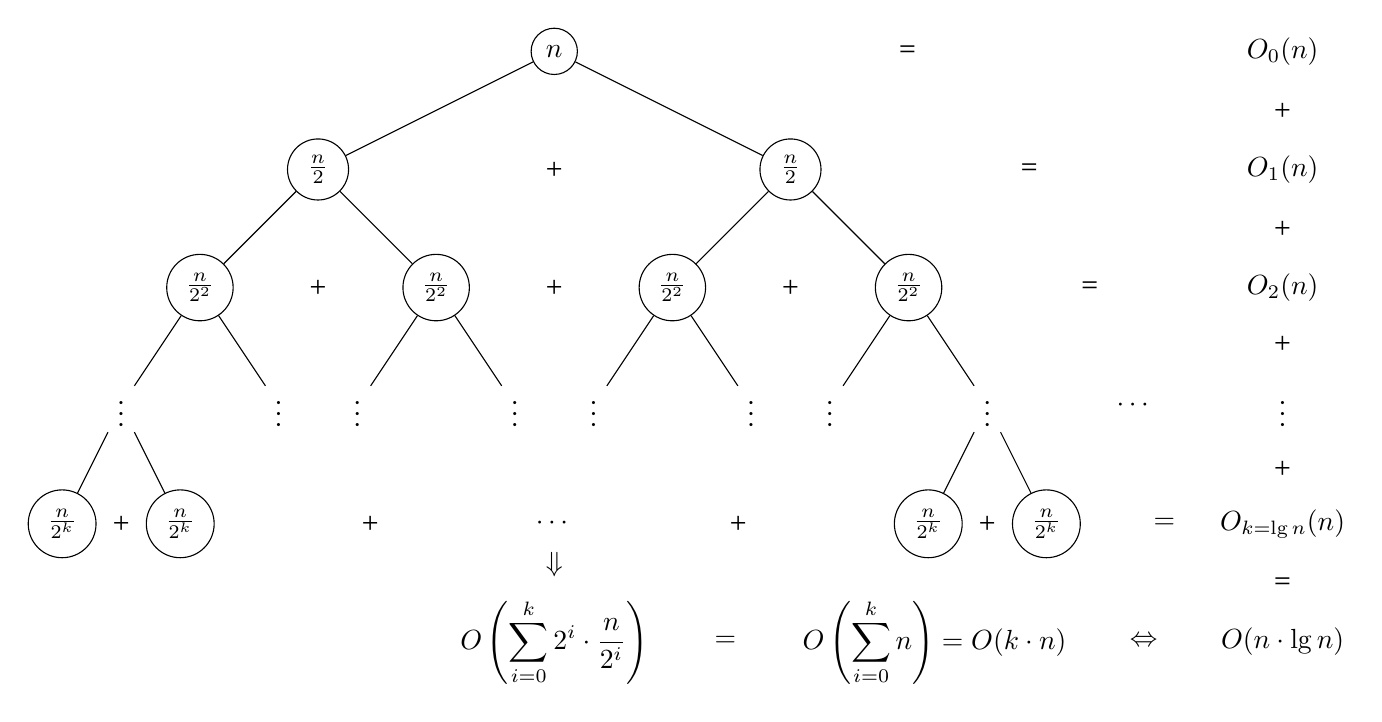
\begin{tikzpicture}[level/.style={sibling distance=60mm/#1}]
\node [circle,draw] (z){$n$}
  child {node [circle,draw] (a) {$\frac{n}{2}$}
    child {node [circle,draw] (b) {$\frac{n}{2^2}$}
      child {node {$\vdots$}
        child {node [circle,draw] (d) {$\frac{n}{2^k}$}}
        child {node [circle,draw] (e) {$\frac{n}{2^k}$}}
      } 
      child {node {$\vdots$}}
    }
    child {node [circle,draw] (g) {$\frac{n}{2^2}$}
      child {node {$\vdots$}}
      child {node {$\vdots$}}
    }
  }
  child {node [circle,draw] (j) {$\frac{n}{2}$}
    child {node [circle,draw] (k) {$\frac{n}{2^2}$}
      child {node {$\vdots$}}
      child {node {$\vdots$}}
    }
  child {node [circle,draw] (l) {$\frac{n}{2^2}$}
    child {node {$\vdots$}}
    child {node (c){$\vdots$}
      child {node [circle,draw] (o) {$\frac{n}{2^k}$}}
      child {node [circle,draw] (p) {$\frac{n}{2^k}$}
        child [grow=right] {node (q) {$=$} edge from parent[draw=none]
          child [grow=right] {node (q) {$O_{k = \lg n}(n)$} edge from parent[draw=none]
            child [grow=up] {node (r) {$\vdots$} edge from parent[draw=none]
              child [grow=up] {node (s) {$O_2(n)$} edge from parent[draw=none]
                child [grow=up] {node (t) {$O_1(n)$} edge from parent[draw=none]
                  child [grow=up] {node (u) {$O_0(n)$} edge from parent[draw=none]}
                }
              }
            }
            child [grow=down] {node (v) {$O(n \cdot \lg n)$}edge from parent[draw=none]}
          }
        }
      }
    }
  }
};
\path (a) -- (j) node [midway] {+};
\path (b) -- (g) node [midway] {+};
\path (k) -- (l) node [midway] {+};
\path (k) -- (g) node [midway] {+};
\path (d) -- (e) node [midway] {+};
\path (o) -- (p) node [midway] {+};
\path (o) -- (e) node (x) [midway] {$\cdots$}
  child [grow=down] {
    node (y) {$O\left(\displaystyle\sum_{i = 0}^k 2^i \cdot \frac{n}{2^i}\right)$}
    edge from parent[draw=none]
  };
\path (q) -- (r) node [midway] {+};
\path (s) -- (r) node [midway] {+};
\path (s) -- (t) node [midway] {+};
\path (s) -- (l) node [midway] {=};
\path (t) -- (u) node [midway] {+};
\path (z) -- (u) node [midway] {=};
\path (j) -- (t) node [midway] {=};
\path (y) -- (x) node [midway] {$\Downarrow$};
\path (v) -- (y)
  node (w) [midway] {$O\left(\displaystyle\sum_{i = 0}^k n\right) = O(k \cdot n)$};
\path (q) -- (v) node [midway] {=};
\path (e) -- (x) node [midway] {+};
\path (o) -- (x) node [midway] {+};
\path (y) -- (w) node [midway] {$=$};
\path (v) -- (w) node [midway] {$\Leftrightarrow$};
\path (r) -- (c) node [midway] {$\cdots$};
\end{tikzpicture}
}
%%%%%%%%%%%%%%%%%%%%%%%%%%%%%%%%%%%%%%%%%%%%%%%%%%%%%%%%%%%%%%%%%%%%%%%%%%%%%%

%%%%%%%%%%%%%%%%%%%%%%%%%%%%%%%%%%%%%%%%%%%%%%%%%%%%%%%%%%%%%%%%%%%%%%%%%%%%%%
\headerbox{Complexity Analysis}{name=complex,column=1}{
%%%%%%%%%%%%%%%%%%%%%%%%%%%%%%%%%%%%%%%%%%%%%%%%%%%%%%%%%%%%%%%%%%%%%%%%%%%%%%
To analyze complexity we assume a sequential algorithm using CUBLAS on a single Kepler K20 GPU and a system of N qubits represented by a float precision state vector.
\begin{equation*}
T_{seq} \propto 4^{N-9}\times(T_{gpu\_mult} +  T_{gpu\_comm})
\end{equation*}
Our MPI parallelized algorithm has the following time complexity
\begin{equation*}
T_{MCQE} \propto l\times T_{mpi\_comm} + \frac{2^{2(N-9)-l}}{4^{l}}\times(T_{gpu\_mult} + T_{gpu\_comm})
\end{equation*}
where $4^{l}$ is the number of MPI ranks available to us.
Thus our speed up is
\begin{equation*}
\frac{l\times T_{mpi\_comm} + 4^{2(N-10-l)}\times(T_{gpu\_mult} + T_{gpu\_comm})}{4^{N-9}\times(T_{gpu\_mult} +  T_{gpu\_comm})}
\end{equation*}
}
%%%%%%%%%%%%%%%%%%%%%%%%%%%%%%%%%%%%%%%%%%%%%%%%%%%%%%%%%%%%%%%%%%%%%%%%%%%%%%

%%%%%%%%%%%%%%%%%%%%%%%%%%%%%%%%%%%%%%%%%%%%%%%%%%%%%%%%%%%%%%%%%%%%%%%%%%%%%%
\headerbox{Expected Results}{name=results,column=1,below=complex}{
%%%%%%%%%%%%%%%%%%%%%%%%%%%%%%%%%%%%%%%%%%%%%%%%%%%%%%%%%%%%%%%%%%%%%%%%%%%%%%
\begin{itemize}
  \item bla
\end{itemize}
}
%%%%%%%%%%%%%%%%%%%%%%%%%%%%%%%%%%%%%%%%%%%%%%%%%%%%%%%%%%%%%%%%%%%%%%%%%%%%%%

%%%%%%%%%%%%%%%%%%%%%%%%%%%%%%%%%%%%%%%%%%%%%%%%%%%%%%%%%%%%%%%%%%%%%%%%%%%%%%
\headerbox{Future Work}{name=future,column=1, below=results}{
%%%%%%%%%%%%%%%%%%%%%%%%%%%%%%%%%%%%%%%%%%%%%%%%%%%%%%%%%%%%%%%%%%%%%%%%%%%%%%
\begin{itemize}
  \item bla
\end{itemize}
}
%%%%%%%%%%%%%%%%%%%%%%%%%%%%%%%%%%%%%%%%%%%%%%%%%%%%%%%%%%%%%%%%%%%%%%%%%%%%%%
\end{poster}
\end{document}

